\documentclass[SE,lsstdraft,authoryear,toc]{lsstdoc}
\input{meta}
% Package imports go here.

% Local commands go here.

%If you want glossaries
%\input{aglossary.tex}
%\makeglossaries
\usepackage{lineno}
\linenumbers

\title{PSF assessment in the field of Abell 360 and shapeHSM shear profile using LSSTComCam data}

% This can write metadata into the PDF.
% Update keywords and author information as necessary.
\hypersetup{
    pdftitle={PSF assessment in the field of Abell 360 and shapeHSM shear profile using LSSTComCam data},
    pdfauthor={C. Combet},
    pdfkeywords={}
}

% Optional subtitle
% \setDocSubtitle{A subtitle}

\author{%
C. Combet, A. Plazas Malagón, S. Fu, P. Adari, I. Dell'Antonio, A. Englert, M. Gorsuch, K. Laliotis, P.-F. Léget, N. Lorenzo, R. Mandelbaum, E. Pedersen, A. von der Linden, Y. Zhang, et al. (TBC)
}

\setDocRef{SITCOMTN-161}
\setDocUpstreamLocation{\url{https://github.com/lsst-sitcom/sitcomtn-161}}

\date{\vcsDate}

% Optional: name of the document's curator
% \setDocCurator{The Curator of this Document}

\setDocAbstract{%
The Rubin LSSTComCam on-sky campaign performed at the end of 2024 provided observations of the Abell 360 galaxy cluster; these data allow a preliminary study of cluster weak lensing analysis using Rubin Data Preview 1 (DP1) data. Among all the steps required for such analyses, accurate modeling of the PSF is essential. This work uses several diagnostics, mostly based on the residuals between the second moments of stars and the PSF model, to characterize the accuracy of the PSF modeling in the A360 field. We find the level of the residuals to be sufficiently low not to hinder the measurement of the tangential shear profile around A360. With a simple source selection process, we demonstrate that outputs of the LSST Science Pipelines can be used to detect the tangential shear profile in Abell 360 at the 3.6$\sigma$ level, and our analysis indicates that contamination from PSF modeling systematics is negligible.
}

% Change history defined here.
% Order: oldest first.
% Fields: VERSION, DATE, DESCRIPTION, OWNER NAME.
% See LPM-51 for version number policy.
\setDocChangeRecord{%
  \addtohist{1}{YYYY-MM-DD}{Unreleased.}{First Last}
}


\begin{document}

% Create the title page.
\maketitle
% Frequently for a technote we do not want a title page  uncomment this to remove the title page and changelog.
% use \mkshorttitle to remove the extra pages
%\mkshorttitle
% ADD CONTENT HERE
% You can also use the \input command to include several content files.

\section{Introduction}
The Rubin LSSTComCam\footnote{\url{https://doi.org/10.71929/rubin/2561361}} on-sky observing campaign (\citeds{RTN-095,SITCOMTN-149})
undertaken at the end-of-year 2024 covered seven fields, among which the low ecliptic latitude Rubin SV 38 7 field. This field contains the Abell 360 (A360) galaxy cluster, an intermediate mass cluster ($M_{500,c} = 6\times 10^{14} \rm{M}_\odot$ from ACT DR5 SZ Cluster Catalog, \citealp{2021ApJS..253....3H}) at z=0.22, that we use as a commissioning demonstrator of cluster weak lensing (WL) studies with data from the Vera C. Rubin observatory. This note focuses on assessing the quality of the PSF modeling in the A360 field, as performed by the Rubin Science Pipeline for the Data Preview 1 (DP1) data release (\citeds{RTN-095}). This note is part of a series studying A360 in order to both stress test the commissioning camera and demonstrate the technical capabilities of the Vera Rubin Observatory; beyond this PSF-related analysis, we study the implementation of cell-based coadds and subsequent use for Metadetect in \citeds{SITCOMTN-162}, source selection of weak lensing galaxies in \citeds{SITCOMTN-163}, photometric calibration in \cite{}, the use of Anacal to produce a cluster shear profile in \citeds{SITCOMTN-164}, and background subtraction in this field and Fornax in \cite{}.




After a description of the data and sofwtare used for this analysis in Section~\ref{sec:data}, we present diagnostics we used to charcterize the PSF model in Section~\ref{sec:tests}. Having found that contamination from PSF modeling systematics should not impact the shear profile measurement around A360, we proceed to the latter in Section~\ref{sec:shear_profile}, before concluding in Section~\ref{sec:conclusion}.

\section{Dataset}
\label{sec:data}
The Rubin SV 38 7 field has been observed in $g$ (44 visits), $r$ (55 visits), $i$ (57 visits) and $z$ (27 visits) (\citeds{RTN-095,SITCOMTN-149}). No $u$ or $y$-band data were collected in that field. The $r$ or $i$-bands are generally used for weak lensing studies (e.g., \citealp{2018MNRAS.481.3170M}); most WL sources tend to have lower SNR in the bluer bands (because of the typical depth of imaging surveys in those bands) and the bluer bands are also more affected by differential chromatic refraction (\citeds{DMTN-017}). For the DP1 analysis of A360 we focus on the $i$-band, which received the most visits in DP1, to measure the shear profile around A360. 

The work presented here uses the DP1 object table, which gathers all the properties of the objects (stars and galaxies) detected in the coadded images, in each band.
All the tests performed hereafter rely on the coadded data from the tracts and patches overlapping with a $1^\circ \times 1^\circ$ square field centered on the Brightest Cluster Galaxy (BCG) of Abell 360, at (ra,dec) = (37.86, 6.98) deg. 


 Figure~\ref{fig:dither} shows the number of images that contributed to the coadds in the field of A360 and was obtained from the \code{i\_inputCount} information available in the object table. The dithering pattern of the observations is clearly visible. 

% \begin{figure}
% 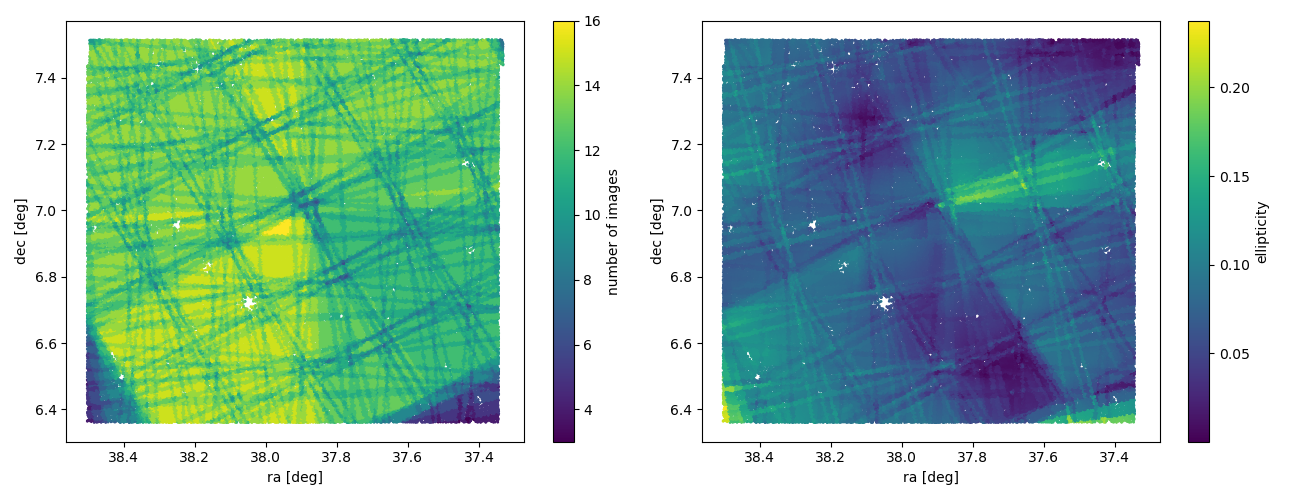
\includegraphics[width=\textwidth]{Figures/psf_ellipticity_visits.png}
% \caption{\emph{Left}: number of images used in the coadded data in the field of A360. \emph{Right}: modulus of the PSF ellipticity in the field. The dithering pattern appears clearly in both figures.\label{fig:dither}}
% \end{figure}

\begin{figure}
\centering'
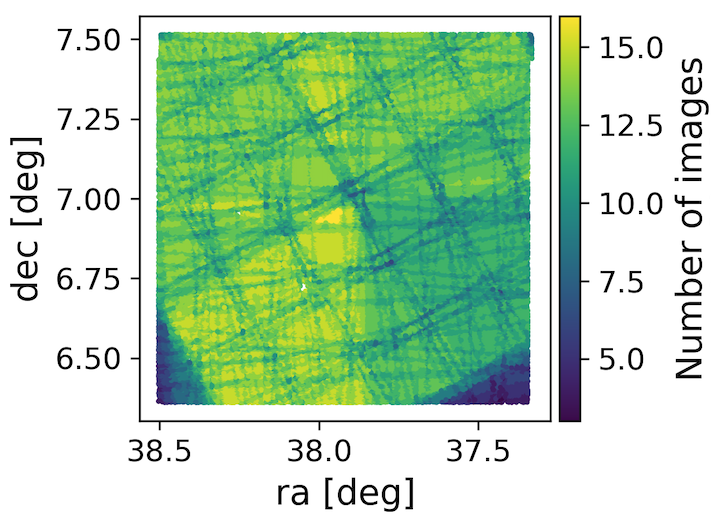
\includegraphics[width=0.5\textwidth]{Figures/nimages.png}
\caption{Number of images used in the coadded data in the field of A360.\label{fig:dither}}
\end{figure}


The PSF modeling of LSSTComCam data was performed using the PSFex \citep{2011ASPC..442..435B} and Piff methods \citep{2021MNRAS.501.1282J}; the latter has been found to be more accurate (\citeds{RTN-095, SITCOMTN-149}) and has been used for the final modeling of DP1. It is therefore the Piff PSF model that is investigated in this note. The PSF estimates are carried out on individual exposures and are then coadded in a self-consistent way with the image coaddition to produce a well-defined coadded PSF. Throughout this note, the term \emph{PSF model} refers to that coadded PSF model rather than to the PSF model from Piff in the individual exposures. 

For each band, the object table includes the second moments of the object surface brightness $I_{xx,xy,yy}$ and second moments of the PSF model $I_{xx,xy,yy}^{\rm PSF}\,$, both measured using the HSM method \citep{2003MNRAS.343..459H, 2005MNRAS.361.1287M, 2018MNRAS.481.3170M}, i.e., they are adaptive second moments determined through iterative fits with an elliptical weighted Gaussian. A flag in the catalog identifies stars that have been used by Piff to build the PSF model; these are termed PSF (used) stars. Additionally, a set of reserved stars (selected with the same criteria as PSF stars, but not used in the fit) are flagged in the catalog for the purpose of PSF testing (e.g., \citealp{2025OJAp....8E..26S}). With that selection, there are 1977 PSF stars and 229 reserved stars at our disposal to run the PSF diagnostics tests below. 

\paragraph*{Software} This work was carried out on the Rubin Science Platform Notebook Aspect at the USDF. The notebooks to generate the figures of this note are available in the note's GitHub repository\footnote{\url{https://github.com/lsst-sitcom/sitcomtn-161}}.
The figures in this note have been produced using the following:
\begin{itemize}
\item \code{repo = '/repo/dp1'}
\item \code {collection = 'LSSTComCam/runs/DRP/DP1/v29\_0\_0/DM-50260'}
\item Science pipeline version: \code{Weekly 2025\_17}
\end{itemize}


\section{PSF properties and diagnostics}
\label{sec:tests}

An accurate PSF model is essential for weak lensing studies. Briefly, PSF model size errors result in an inaccurate correction for the dilution of the galaxy shear by the PSF convolution, which causes a coherent multiplicative bias in weak lensing shear; PSF model shape errors result in an inaccurate correction for the PSF shape, causing a coherent additive bias in weak lensing shear. Evaluating the performance of the PSF model on both aspects required comparing the PSF model to the measurements of the PSF and reserved sets of stars. We refer the reader to the PSF-related studies carried out to validate the shape catalogs of stage~III galaxy surveys (e.g. \citealp{2018PASJ...70S..25M, 2022PASJ...74..421L} for HSC; \citealp{2016MNRAS.460.2245J, 2018MNRAS.481.1149Z, 2021MNRAS.504.4312G} for DES) for a more comprehensive view than what we cover in this note.

The second moments $I_{xx,xy,yy}$ measured on the objects and of the PSF model lie at the core of shape measurements used in weak lensing analyses. We refer the reader to \citet{2014ApJS..212....5M} for a pedagogical overview and provide here the main quantities needed in this note.   

From the second moment matrix expressed in the (x,y) frame of the tracts, we define the trace 
\begin{equation}
T = I_{xx} + I_{yy}\;,
\end{equation}
that provides an estimate of the size of the object.

In addition, the shape of an object can be described by its complex ellipticity, $e=e_1+i e_2$, the components of which relates to the the second moments as
\begin{eqnarray}
  e_1 &=& (I_{xx} - I_{yy})/T \\
  e_2 &=& 2 I_{xy} / T\;.
\end{eqnarray}

From these, we compute the residuals between the measurements for the set of PSF (or reserved) stars and that of the PSF model at their locations.  Namely,
\begin{eqnarray}
\delta e_1 &=& e_1^{\rm meas} - e_1^{\rm model}, \, \delta e_2 = e_2^{\rm meas} - e_2^{\rm model}\\
\delta T &=& T^{\rm meas} - T^{\rm model} 
\end{eqnarray}

The ellipticity can equivalently be written as $e = |e| \exp(2i\theta)$, where $|e|$ is the modulus of the ellipticity and $\theta$ the orientation of the major axis of the ellipse with respect to the x axis. They are expressed from $e_1$ and $e_2$ as follows
\begin{equation} 
|e| = \sqrt{e_1^2 + e_2^2}
\label{eq:modulus}
\end{equation}
\begin{equation}
\theta = 0.5 \times \arctan(e_2/e_1)\;.
\label{eq:theta}
\end{equation}


Before looking into the residuals in the next section, Figure~\ref{fig:T_and_e} displays the PSF model trace $T$ (left) and the modulus of ellipticity $|e|$ (right) in the field. While the mean ellipticity across the field is ~0.07, there are several areas where the PSF ellipticity reaches significant values. This could be investigated further by checking the PSF at the individual visit level; this goes however beyond the scope of this technote which aims at checking, in the next section, whether the PSF modeling is sufficient for the purpose of measuring a lensing profile around A360.



\begin{figure}
\centering
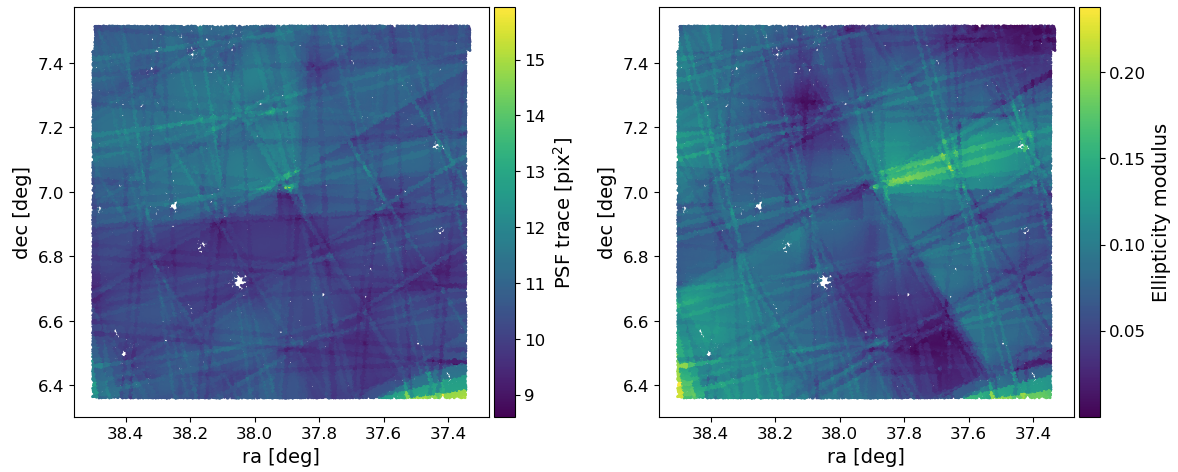
\includegraphics[width=\textwidth]{Figures/T_and_e.png}
\caption{\emph{Left}: PSF model trace across the field. \emph{Right}: modulus of the PSF ellipticity in the field. \label{fig:T_and_e}}
\end{figure}  


\subsection{PSF residuals - distributions and whisker plots}
To assess the performance of the PSF model, a first test consists in comparing the normalized distribution of the residuals defined above, for the PSF and reserved stars, to check for a possible overfitting of the PSF model (e.g., \citealp{2025OJAp....8E..26S}). As can be seen in Figure~\ref{fig:residual_distrib} (left and middle panels), the ellipticity residuals peak around zero and extend to $\sim 0.02$. The right panel shows the relative residuals of the trace, peaking around zero and not exceeding beyond $\sim 5 \%$. The residuals obtained from the PSF stars and reserved stars behave similarly, so there is no indication of any overfitting of the PSF model.

\begin{figure}
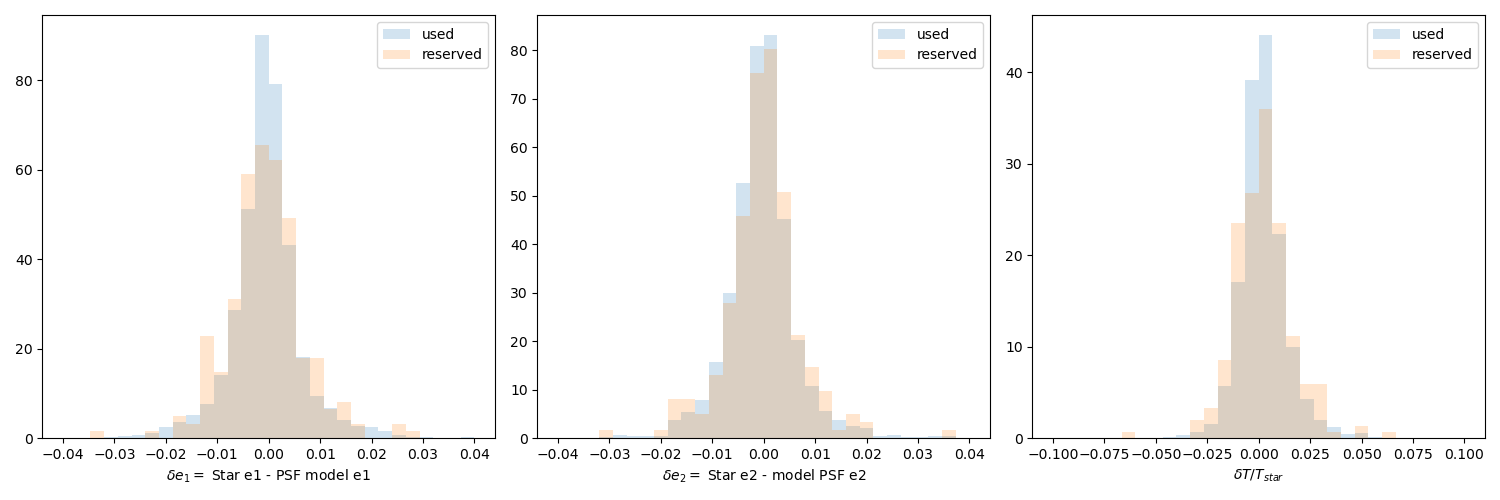
\includegraphics[width=\textwidth]{Figures/residual_histograms.png}
\caption{Normalised distributions of the ellipticity residuals $\delta e_1$ (left), $\delta e_2$ (right), and of the relative residuals $\delta T/T$ (right). The distributions are shown for the PSF (blue) and reserved (orange) sets of stars. \label{fig:residual_distrib}}
\end{figure}

Following \citet{2004MNRAS.353..529H, 2018PASJ...70S..25M}, a PSF model size error $\delta T$ yields a shear calibration (multiplicative bias) uncertainty $\delta m = -(R_2^{-1} -1)\; \delta T/T$, where $R_2$ is the so-called resolution factor\footnote{The resolution factor, $R_2 = 1 -\frac{T^{\rm PSF}}{T_{\rm gal}}$, tends to zero for poorly-resolved galaxies and to 1 for well-resolved ones.}. In the right panel of Figure~\ref{fig:residual_distrib}, the mean value of the PSF trace residuals for the reserved stars is $\langle \delta T/T \rangle = 0.002$. Combined with a conservative mean value\footnote{For the source galaxy sample used in Section~\ref{sec:shear_profile}, that were requesting $R_2 > 0.3$, we find $\langle R_2^{-1} -1 \rangle = 0.96$.} 
$\langle R_2^{-1} -1 \rangle = 1$, we get $\langle \delta m \rangle = 0.002$. These numbers are roughly on par with the typical requirements for the Y1 DESC weak lensing ($3 \times 2$-point) analyses \citep{2018arXiv180901669T}, which are more demanding than the use case of galaxy cluster lensing we are considering here.


\begin{figure}
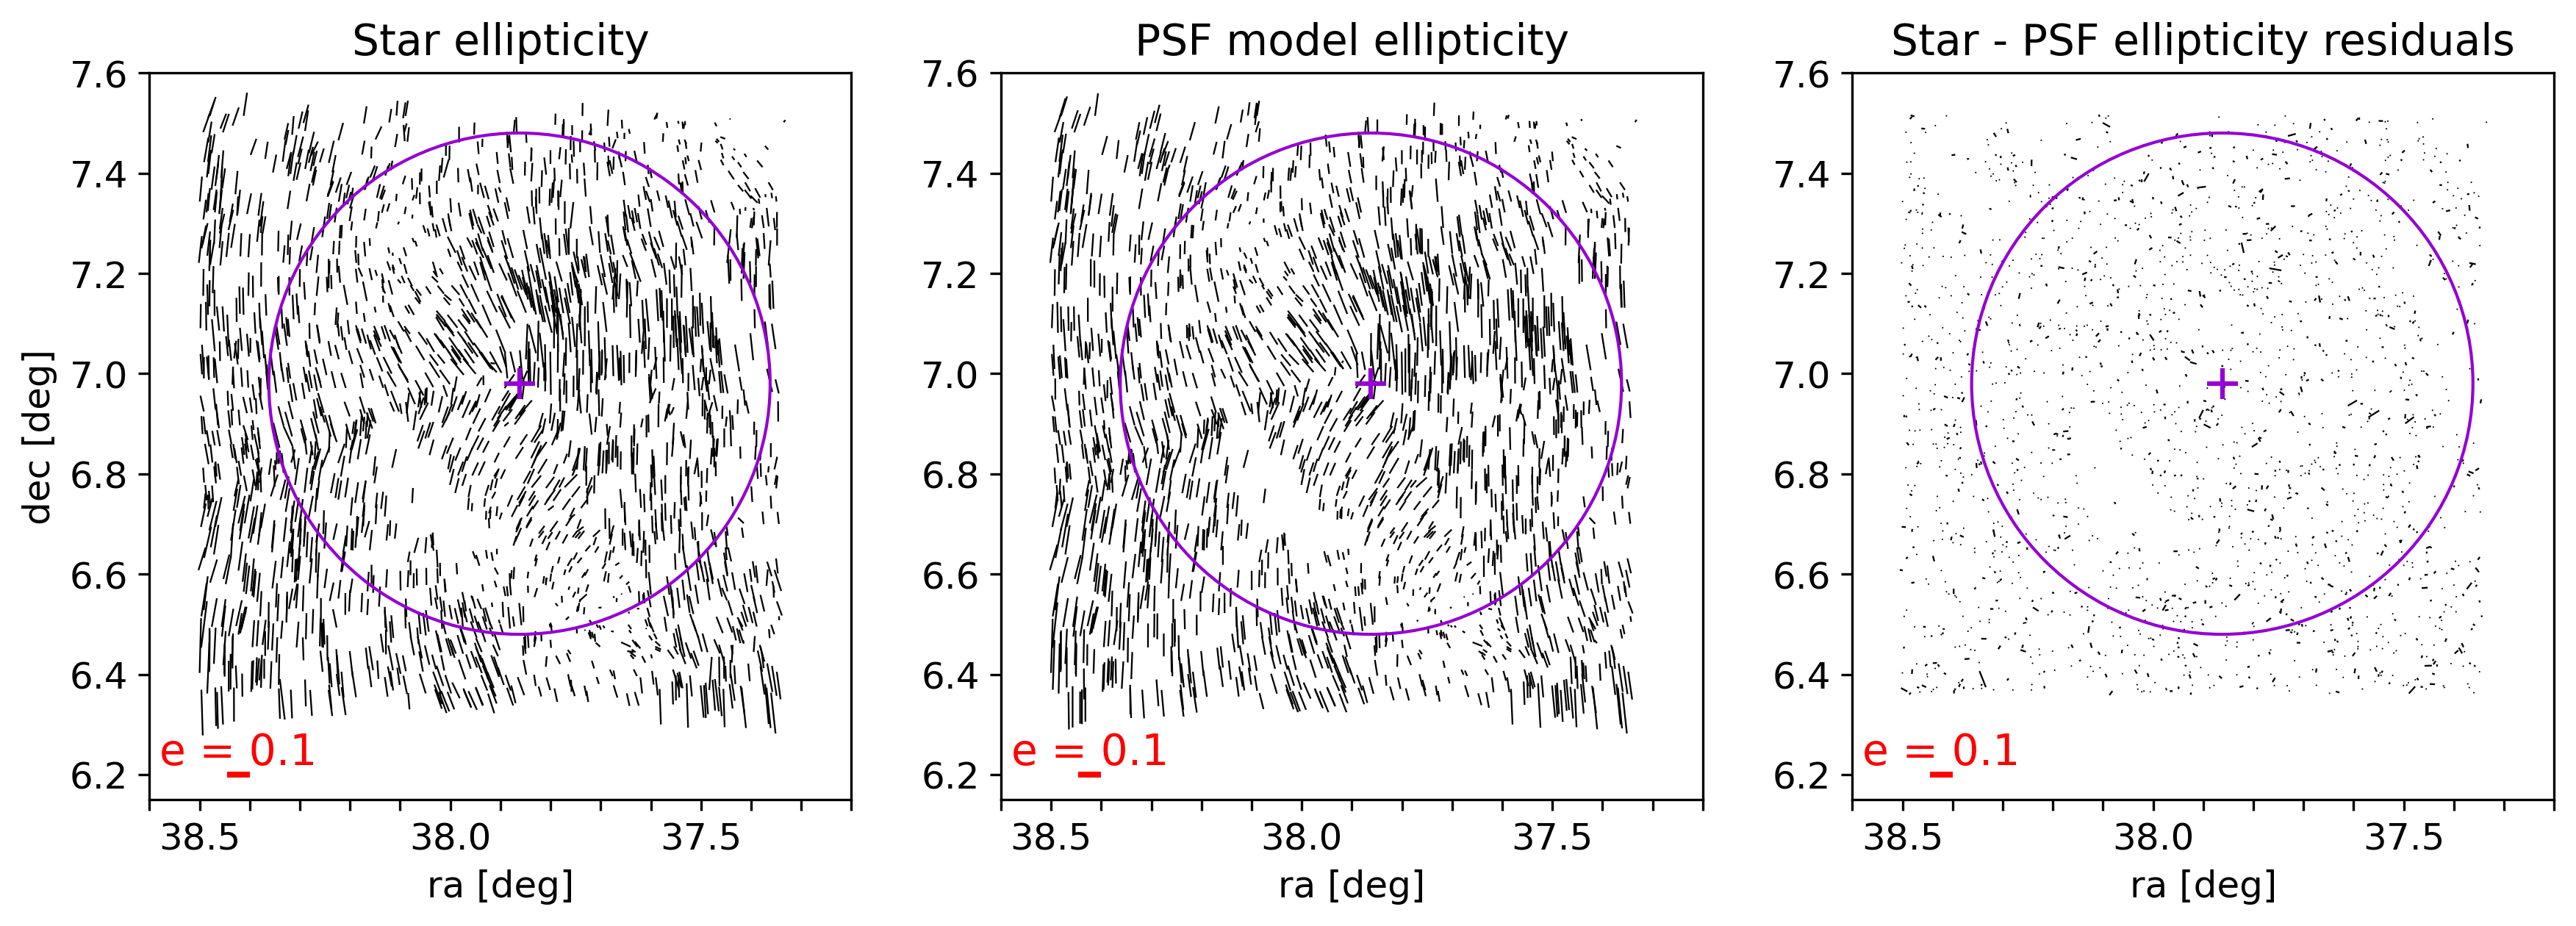
\includegraphics[width=\textwidth]{Figures/whiskers_used_big.png}
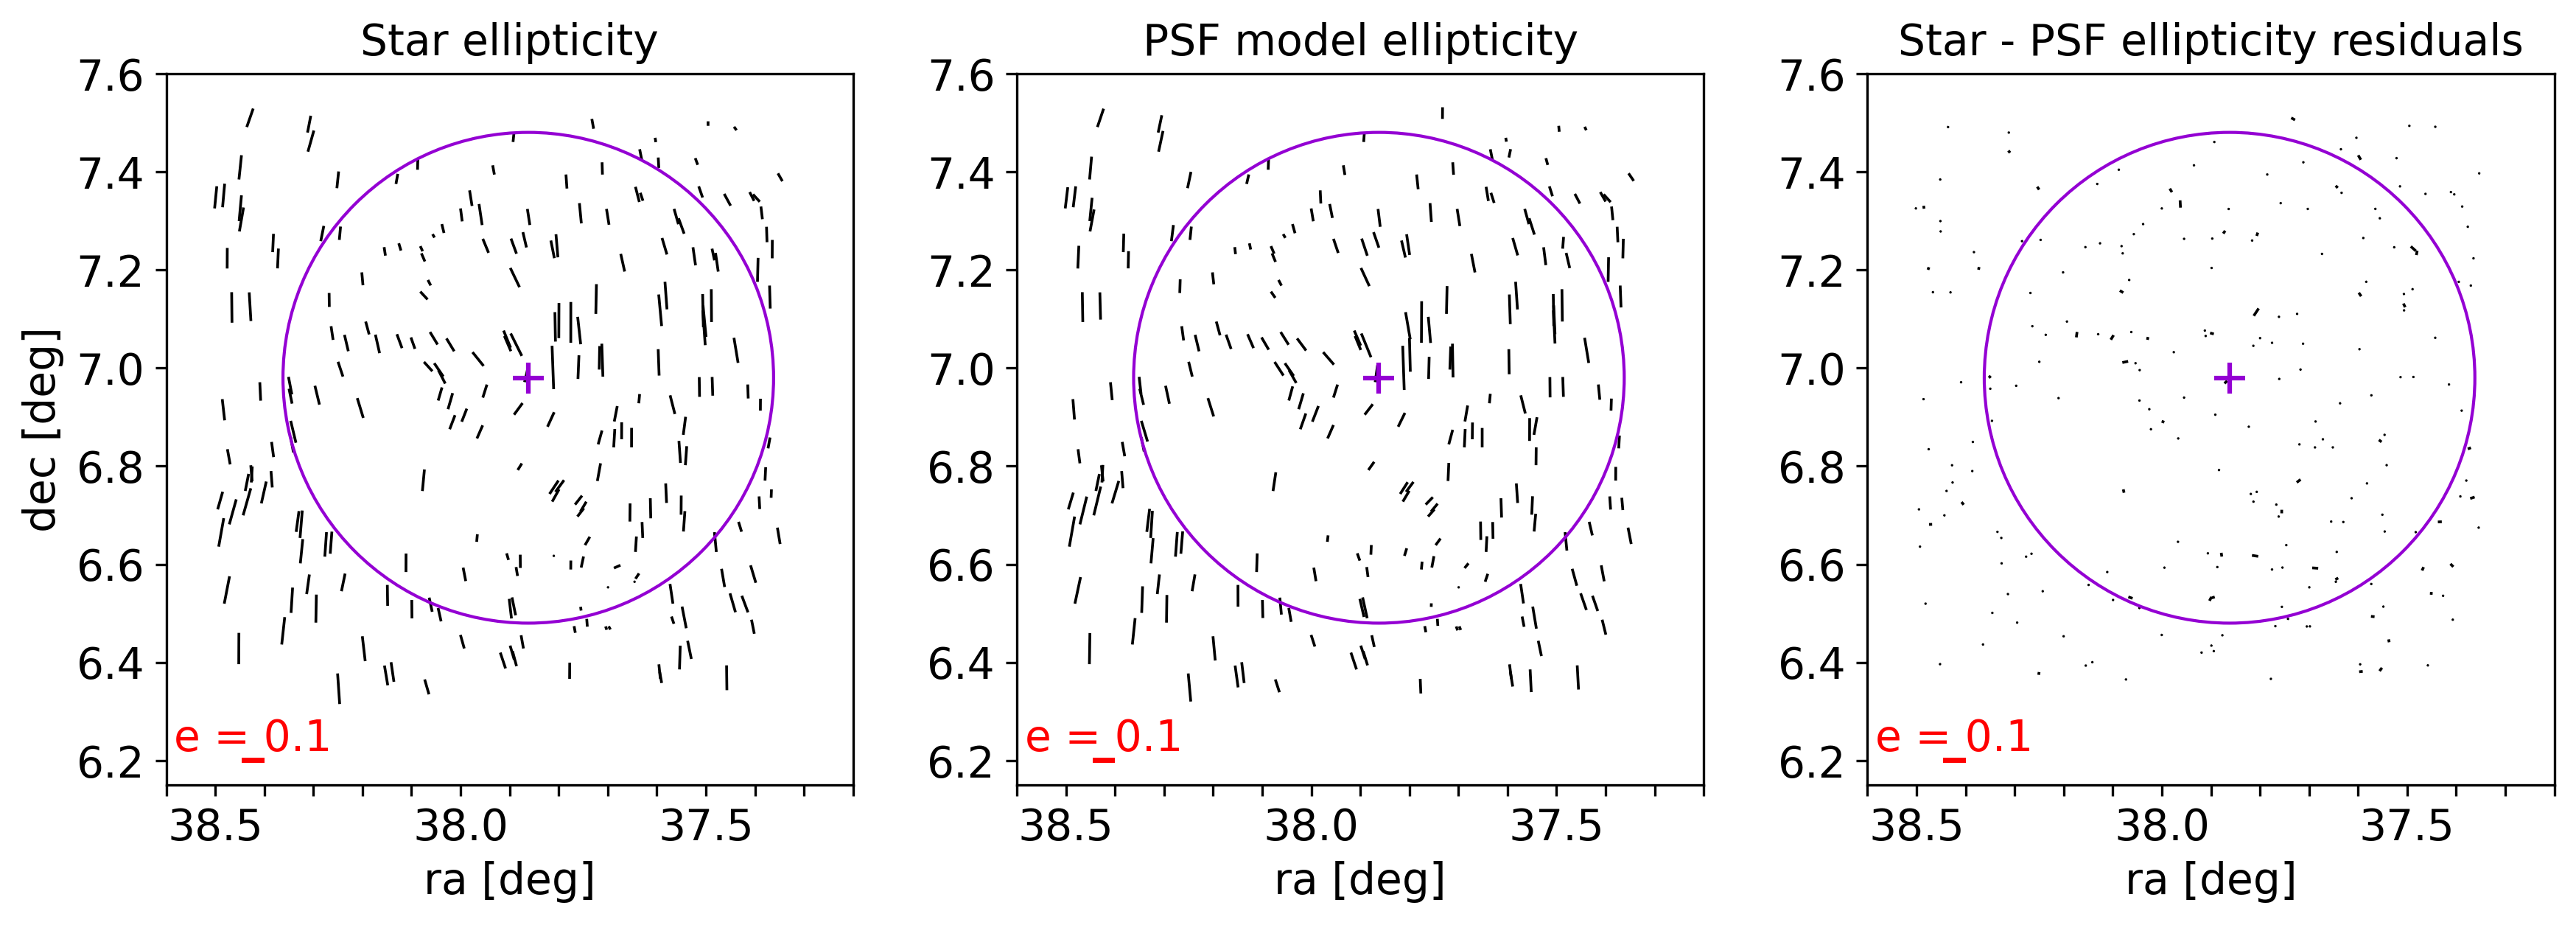
\includegraphics[width=\textwidth]{Figures/whiskers_reserved_big.png}
\caption{Whisker plots for the PSF (top) and reserved stars (bottom) obtained for the measurements (left), PSF model (middle) and the residuals (right). The size of the whiskers is proportional to the ellipticity modulus and the orientation gives the direction of the major axis of the ellipse. The circle corresponds to a $0.5^\circ$  field around the cluster’s BCG, i.e., corresponding to $\sim 6$~Mpc at the cluster's redshift (roughly the field we aim the WL measurements at).\label{fig:whiskers}}
\end{figure}

Figure~\ref{fig:whiskers} shows the variation of the PSF ellipticity and residuals across the field of A360. Each whisker is oriented according the direction of the ellipse major axis ($\theta$, Eq.(\ref{eq:theta})) and its length is proportional to the ellipticity modulus ($|e|$, Eq.(\ref{eq:modulus})); this is done for the PSF stars (top row) or reserved stars (bottom row). The left panel corresponds the measurements on the star themselves, the middle panel shows the corresponding PSF model, and the residuals are displayed in the right panel. A reference whisker is given for an ellipticity $|e| = 0.1$. Visually, the residuals (right panel) display no coherent pattern, which combined with the fact that they appear symmetrically distributed around zero in Figure~\ref{fig:residual_distrib}, suggests a good performance of the PSF model. We will quantify whether this is satisfactory and sufficient for the purpose of measuring the shear signal around A360 below.


\subsection{PSF residuals - tangential shear profile}

An important diagnostic for cluster weak lensing is to evaluate the contribution of the PSF residuals to the tangential shear signal. To do so, we compute the tangential component of the residual ellipticity, $\delta e_t$, analogously to the way the tangential shear signal is estimated around a cluster, namely 
\begin{equation}
\delta e_t = - \delta e_1  \cos(2 \phi) - \delta e_2  \sin(2 \phi),
\end{equation}
where $\phi$ is the position angle (with respect to the cluster center) at the location of the computed residuals. %\footnote{In the notebook supporting this note, this is done using the DESC CLMM code \citep{2021MNRAS.508.6092A}. To do so without relying on CLMM, we refer the reader to the following Rubin DP1 tutorial notebook: \url{https://dp1.lsst.io/tutorials/notebook/304/notebook-304-1.html}}. 
 This provides an estimate of the additive bias in the tangential shear signal resulting from residuals in the PSF modeling.

Figure~{\ref{fig:res_profile}} shows the corresponding binned radial profile (and corresponding statistical errors) as a function of the angular separation from the cluster center. The profile for PSF stars shows smaller error bars because of the larger number compared to the reserved set of the stars. The profiles are broadly consistent with zero on all scales given the errorbars (e.g, p-value $p=0.2$ for the reserved set of stars). 

\begin{figure}
\centering
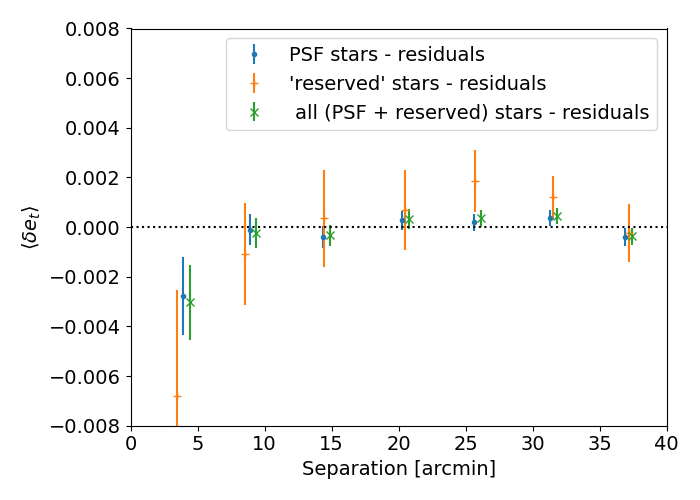
\includegraphics[width=0.7\textwidth]{Figures/residual_tan_profile_CLMM.png}
\caption{Binned tangential profile of the ellipticity residuals for the PSF stars (blue circle), for the reserved stars (orange plus sign marker), and for both sets together (green cross). The error bars correspond to the statistical uncertainties.\label{fig:res_profile}}
\end{figure}


\subsection{PSF rho-statistics}
The $\rho$-statistics \citep{2010MNRAS.404..350R, 2016MNRAS.460.2245J} are a set of two-point correlation functions involving PSF ellipticity and size residuals, $\delta e$ and $\delta T$. They quantify spatially-correlated errors in PSF modeling and contributions from PSF leakage, that yield additive biases to the shear estimation. These statistics are particularly relevant to cosmic shear studies and specific requirements have been established in this context in the litterature (e.g., \citealp{2018PASJ...70S..25M, 2022PASJ...74..421L} for HSC,  \citealp{2018MNRAS.481.1149Z, 2021MNRAS.504.4312G} for DES). 

We use the LSST Science Pipelines \code{analysis\_tools}\footnote{\url{https://pipelines.lsst.io/v/daily/modules/lsst.analysis.tools}} implementation to compute the $\rho$-statistics, which internally relies on the TreeCorr software package \citep{2015ascl.soft08007J} for the correlation function calculations. The definitions of the $\rho$-statistics as calculated by \code{analysis\_tools} are documented in the LSST science pipelines and include the $\rho_1$ to $\rho_5$ originally introduced by \citet{2010MNRAS.404..350R, 2016MNRAS.460.2245J}, as well as $\rho_{3^\prime}$ defined in the context of cluster analysis by \citet{2015MNRAS.449.2219M}.

We used the set of reserved stars to calculate the rho stfatistics in the $i$-band, up to 40 arcmin (i.e. the region of interest for A360 WL measurement) and display the results in Figure~\ref{fig:rho_stat}. We consider the Y1 and Y3 HSC requirements for cosmic shear (see Figure~26 in \citealp{2022PASJ...74..421L}) as a first point of comparison to the $\rho_1$ to $\rho_5$-statistics computed here, noting that cluster lensing would generally be less demanding that cosmic shear because of the order of magnitude larger signal we expect. 



\begin{figure}
\centering
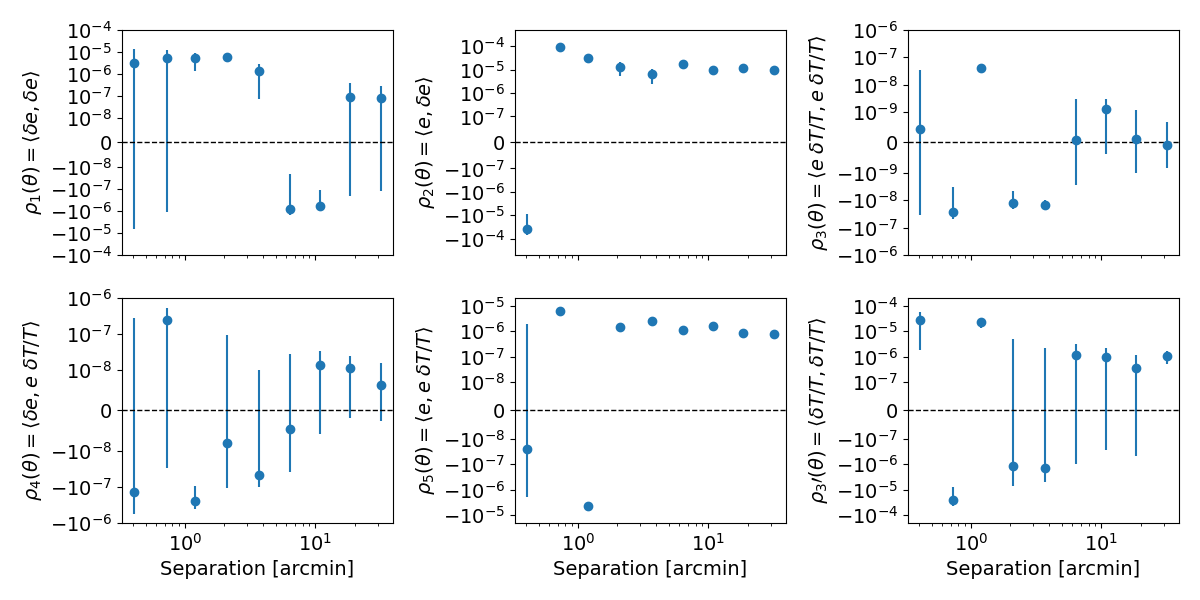
\includegraphics[width=\textwidth]{Figures/rho_stat_noband.png}
\caption{The various $\rho$-statistics correlations as a function of separation, as produced by the Rubin \code{AnalysisTools} software.\label{fig:rho_stat}}
\end{figure}

In the field of A360, with this commissioning data set, we find that $\rho_1$ and $\rho_2$ are typically at the level of the Y1 HSC cosmic shear requirements, while $\rho_3$, $\rho_4$, and $\rho_5$ already fulfill the more stringent HSC Y3 requirements \footnote{$\rho_1$, $\rho_2$ and $\rho_{3^\prime}$ are also well below the tolerances estimated in the early work of \citet{2015MNRAS.449.2219M} to measure cluster WL signals with the DES science verification data.}. We are therefore confident that the corresponding additive biases would be sufficiently low for the WL analysis of A360\footnote{Figure~26 in \citet{2022PASJ...74..421L} used as comparison started from 3~arcmin only, and so more specific cluster-related considerations may be needed for the smaller scales down to which we measure cluster weak lensing.}.


% For this cluster, the size scale is a few arcminutes. In the $\rho_2$ plot, we see that the PSF shape modeling bias (square root of $\rho_2$) is $\lesssim 10^{-3}$ at the cluster length scale that we are interested in. We note that the typical shear is $\sim 3\times10^{-2}$ (see Figure~\ref{fig:shear_profile}). Thus, the PSF modeling bias is $\sim <0.3/3=10$, i.e. one order of magnitude lower than the shear. This is consistent with our previous conclusion, which means the bias is sufficiently small in our shear measurement.


\section{HSM tangential and cross shear profile around A360 from simple color-cut selection}
\label{sec:shear_profile}

From the tests above, it appears that the PSF modeling in the A360 field is sufficiently accurate not to hinder a first attempt at measuring the tangential and cross shear profiles around that cluster. The cross shear profile, which has no contribution from lensing when azimuthally averaged around the cluster center, is a particularly useful null test to highlight remaining systematics effects. We therefore proceed to do so, using the \code{shapeHSM} ellipticities readily available in the object table (other shape measurements methods, such as \code{Metadetect} or \code{Anacal} will be explored elsewhere; see \citeds{SITCOMTN-162} for the \code{Metadetect} analysis). 

For this preliminary work, we use a visual inspection of the $r-i$ versus $r$ color-magnitude diagram to select and remove red sequence galaxies from the sample. Source selection in other colors and using photoz is explored more thoroughly in \citeds{SITCOMTN-163}. 
Given that the LSSTComCam field of A360 reaches roughly similar depth as HSC Y1 and uses a similar pipeline, we use the HSC Y1 lensing quality cuts; with these cuts, the source galaxy density is $n_{\rm gal}\approx 7-8\;{\rm arcmin}^{-2}$.  With then use the shear calibration procedure\footnote{The script to applied the calibration is available at \url{https://github.com/PrincetonUniversity/hsc-y1-shear-calib}. It was slightly adapted to use the column names from the object table.} \citep{2018MNRAS.481.3170M} to convert the $e_1$ and $e_2$ ellipticities into $g_1$ and $g_2$ shear estimates. 

Once the calibration has been applied, we use the DESC CLMM package \citep{2021MNRAS.508.6092A} to compute the tangential and cross reduced shear radial profiles with statistical error bars, displayed in Figure~\ref{fig:shear_profile}. The physical distance on the x-axis is obtained from the angular separation assuming a default cosmology ($\Omega_m=0.3$, $h=0.7$), and ranges from 0.5 Mpc to 6 Mpc (to match the circular 0.5 deg field highlighted in the PSF diagnostic plots at the upper end, and to avoid the cluster inner regions known to be affected by other sources of biases such as miscentering and sample contamination). 

\begin{figure}
\centering
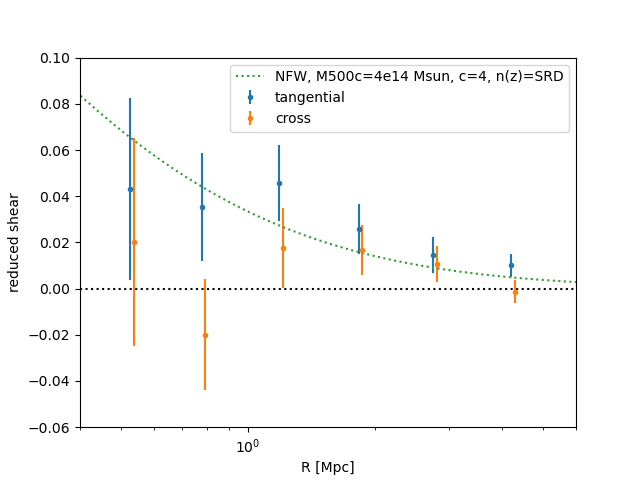
\includegraphics[width=0.7\textwidth]{Figures/shear_profile.png}
\caption{Binned tangential (blue) and cross (orange) reduced shear profile around A360. The green dashed line shows the expected signal for a NFW halo of mass similar to that of A360, a concentration $c=4$, and (wrongly) assumes the Y10 redshift distribution $n(z)$ from the DESC Science Requirement document. \label{fig:shear_profile}}
\end{figure}


Due to the small galaxy sample size, the WL measurements around individual clusters are inherently very noisy, as can be seen from the figure. Nonetheless, the cross shear signal, in orange, appears to scatter around zero over the whole redshift range. We also see a trend for a positive tangential shear signal, increasing towards the inner regions. Computing the $p$-values for both the tangential and cross signals, we find evidence of a tangential shear signal around the cluster at $3.6\sigma$ significance ($p = 1.4 \times 10^{-4}$), while the cross shear is consistent with zero ($p = 0.87$).

While this analysis is too preliminary to conclude on the robustness of the measured signal, we overplot in dashed green the expected signal from a NFW halo with the mass of A360, an assumed concentration $c=4$, and a (wrongly) assumed Y10 source redshift distribution\footnote{The Y10 SRD n(z) is pre-coded and readily available in CLMM.} from the DESC Science Requirements Document \citep{2018arXiv180901669T}; the actual photometric redshift distribution in that field (and of the DP1 data) is explored in \citeds{SITCOMTN-154}. We see that the measured tangential shear is in the ballpark of what one could expect with these simplifying assumptions, although more work is required to robustify this result.


\section{Conclusion}
\label{sec:conclusion}
We have checked the PSF model in the field of the galaxy cluster A360, which was observed in the low ecliptic latitude field of the Rubin 2024 LSSTComCam campaign. While the PSF ellipticity reaches values as high as >~0.2 in the coadded data, we find that the model is able to capture and correct the PSF, at a level sufficient to enable the measurement of the shear profile around A360, which we detect with a 3.6$\sigma$ significance.


\appendix
% Include all the relevant bib files.
% https://lsst-texmf.lsst.io/lsstdoc.html#bibliographies
\section{References} \label{sec:bib}
\renewcommand{\refname}{} % Suppress default Bibliography section
\bibliography{local,lsst,lsst-dm,refs_ads,refs,books}

% Make sure lsst-texmf/bin/generateAcronyms.py is in your path
\section{Acronyms} \label{sec:acronyms}
\addtocounter{table}{-1}
\begin{longtable}{p{0.145\textwidth}p{0.8\textwidth}}\hline
\textbf{Acronym} & \textbf{Description}  \\\hline

DESC & Dark Energy Science Collaboration \\\hline
DM & Data Management \\\hline
DMTN & DM Technical Note \\\hline
DP1 & Data Preview 1 \\\hline
DRP & Data Release Processing \\\hline
HSC & Hyper Suprime-Cam \\\hline
HSM & Hierarchical Storage Management \\\hline
LSST & Legacy Survey of Space and Time (formerly Large Synoptic Survey Telescope) \\\hline
LSSTComCam & Rubin Commissioning Camera \\\hline
PSF & Point Spread Function \\\hline
RTN & Rubin Technical Note \\\hline
SE & System Engineering \\\hline
SNR & Signal to Noise Ratio \\\hline
SV & Science Validation \\\hline
TBC & To Be Confirmed \\\hline
USDF & United States Data Facility \\\hline
WL & Weak gravitational Lens cosmic shear \\\hline
\end{longtable}

% If you want glossary uncomment below -- comment out the two lines above
%\printglossaries





\end{document}
